\documentclass[12pt,unicode]{beamer}

\newcommand{\insertministry}[0]{\ministry}
\newcommand{\insertchief}[0]{\chief}
\newcommand{\insertdone}[0]{\done}
\newcommand{\insertwhochiefed}[0]{\whochiefed}

\defbeamertemplate*{title page}{customized}[1][]
{
  \usebeamerfont{ministry}\insertministry\par
  \bigskip
  \bigskip
  \usebeamerfont{title}\inserttitle\par
  \usebeamerfont{subtitle}\usebeamercolor[fg]{subtitle}\insertsubtitle\par
  \bigskip
  \begin{table}
    \begin{tabular}{ p{5cm} r }
      \usebeamerfont{author}\insertdone   & \usebeamerfont{author}\insertwhochiefed \\
      \usebeamerfont{author}\insertauthor & \usebeamerfont{author}\insertchief \\
    \end{tabular}
  \end{table}
  \par
  \usebeamerfont{date}\insertdate\par
  \usebeamercolor[fg]{titlegraphic}\inserttitlegraphic
}

\usepackage[utf8]{inputenc}
\usepackage[T2A]{fontenc}
\usepackage[english,russian]{babel}

\usepackage{pscyr}          % Cyrillic fonts

\pretolerance=10000         % disable wordwrapping

\usepackage{tabularx}
\newcolumntype{C}[1]{>{\centering\let\newline\\\arraybackslash\hspace{0pt}}m{#1}}
\newcolumntype{L}[1]{>{\raggedright\let\newline\\\arraybackslash\hspace{0pt}}m{#1}}
\newcolumntype{R}[1]{>{\raggedleft\let\newline\\\arraybackslash\hspace{0pt}}m{#1}}

% Стиль презентации
\usetheme{Szeged} 
%\usetheme{Singapore}
%\usefonttheme[]{serif}
\usefonttheme{professionalfonts}

\setbeamerfont{ministry}{size=\large}
%\usecolortheme{lily}
\beamertemplatenavigationsymbolsempty %remove navigation symbols

\title{Исследование методов формирования нелинейных узлов замен блочных симметричных шифров}
\author{ст.гр. БИКСм-12-1 \newlineФролов В.В.}

\begin{document}

\def\ministry{Министерство образования и науки Украины}
\def\done{Выполнил}
\def\whochiefed{Руководитель}
\def\chief{д.т.н., проф. Кузнецов А.А.}
\date{}

% Создание заглавной страницы
\frame{\titlepage} 
% Автоматическая генерация содержания


\begin{frame}{Задачи}

    \begin{itemize}

        \item Анализ методов формирования нелинейных узлов замен.

        \item Исследование и улучшение метода имитации отжига.

        \item Практические оценки повышения стойкости шифров (DES, MacGuffin,
        ГОСТ 28147-89) с использованием оптимальных S-блоков.

        \item Оценка производительности метода имитации отжига.

    \end{itemize}

\end{frame} 


\begin{frame}{Классификация методов формирования нелинейных узлов замен}

    \begin{table}
        \def\arraystretch{1.5}
        \begin{tabular}{ L{3cm} | L{3.6cm} | L{3.3cm} }
            \bf Методы случайной генерации  & \bf Методы алгебраического построения & \bf Методы эвристического поиска \\ \hline\hline
            Случайная генерация с фильтрацией & Степенное отображение в поле & Метод имитации отжига \\ \hline
            Побитовые методы & Инверсия в поле с афинными преобразованиями & Генетические алгоритмы \\
        \end{tabular}
    \end{table}

\end{frame} 


\begin{frame}{Метод имитации отжига}

    \begin{itemize}

        \item Является универсальным оптимизационным алгоритмом.

        \item Представляет собой вероятностный вычислительный поиск оптимальных нелинейных узлов замен.

        \item Основывается на пошаговом улучшении S-блока за счёт постепенного
        снижения температурного показателя.

        \item Используется специальная ценовая функция.

    \end{itemize}

\end{frame}


\begin{frame}{Критерии отбора нелинейных узлов замен}

    \begin{itemize}

        \item Нелинейность должна быть максимизирована.

        \item При равной нелинейности автокорреляция должна быть минимизирована.

        \item Дополнительные шифрозависимые критерии.

    \end{itemize}

\end{frame}


\begin{frame}{S-блоки шифра DES}

    \begin{itemize}
        
        \item В DES используются S-блоки $6 \times 4$, $GF(2^6) \rightarrow GF(2^4)$

        \item К S-блокам DES выдвигается дополнительных 11 (8~основных и 3 дополнительных) критериев

        \item Метод имитации отжига формирует S-блоки с оптимальными показателями нелинейности ($NL = 24$) и автокорреляции ($AC = 24$)
        
        \item Метод имитации отжига не учитывает критерии DES

    \end{itemize}

\end{frame}


\begin{frame}{S-блоки шифра MacGuffin}

    \begin{itemize}
        
        \item S-блоки $6 \times 4$, $GF(2^6) \rightarrow GF(2^2)$
        \item Нет дополнительных критериев, ограничивающих множество S-блоков

    \end{itemize}

\end{frame}


\begin{frame}{Сравнительный анализ исходных и оптимальных S-блоков MacGuffin}

    \begin{table}
        \def\arraystretch{1.5}
        \begin{tabular}{ L{4.1cm} | L{2.7cm} | L{2.7cm} }
        \bf Криптографические показатели & \bf Исходные S-блоки & \bf Оптимальные S-блоки \\ \hline
        Нелинейность ($NL$) & 16 .. 20 & 24 \\ \hline
        Автокорреляция ($AC$) & 32 .. 64 & 16 \\ \hline
        $\Delta$-разность & 32 .. 36 & 24 \\ \hline
        Лучшая линейная аппроксимация & 12 .. 16 & 8 \\ \hline
        \end{tabular}
    \end{table}

\end{frame}

\begin{frame}{S-блоки шифра ГОСТ 28147-89}

    \begin{itemize}
        
        \item Биективные S-блоки $4 \times 4$, $GF(2^4) \rightarrow GF(2^4)$

        \item Для оценки эффективности использовались оценки практической
        стойкости относительно верхней границы вероятности криптоанализа,
        полученные в работах Алексейчука и Ковальчука

        \item $M_D$ --- оценка вероятности дифференциального криптоанализа

        \item $M_L$ --- оценка вероятности линейного криптоанализа

    \end{itemize}

\end{frame}


\begin{frame}{Сравнительный анализ ЦБ РФ и оптимальных S-блоков ГОСТ 28147-89}

    \begin{table}
        \def\arraystretch{1.4}
        \begin{tabular}{ L {4.1cm} | L{2.7cm} | L{2.7cm} }
        \bf Криптографические показатели & \bf S-блоки ЦБ~РФ & \bf Оптимальные S-блоки \\ \hline
        Нелинейность ($NL$) & $2$ (лишь один S-блок имеет $NL = 4$) & $4$ \\ \hline
        Автокорреляция ($AC$) & $16$ & $8$ \\ \hline
        $M_D$ & $2^{-34.02}$ & $2^{-66}$ \\ \hline
        $M_L$ & $2^{-35.24}$ & $2^{-42}$ \\ \hline
        \end{tabular}
    \end{table}

\end{frame}

\begin{frame}{Эффективность ГОСТ~28147-89. Стойкость к дифференциальному криптоанализу}

    \begin{figure}
        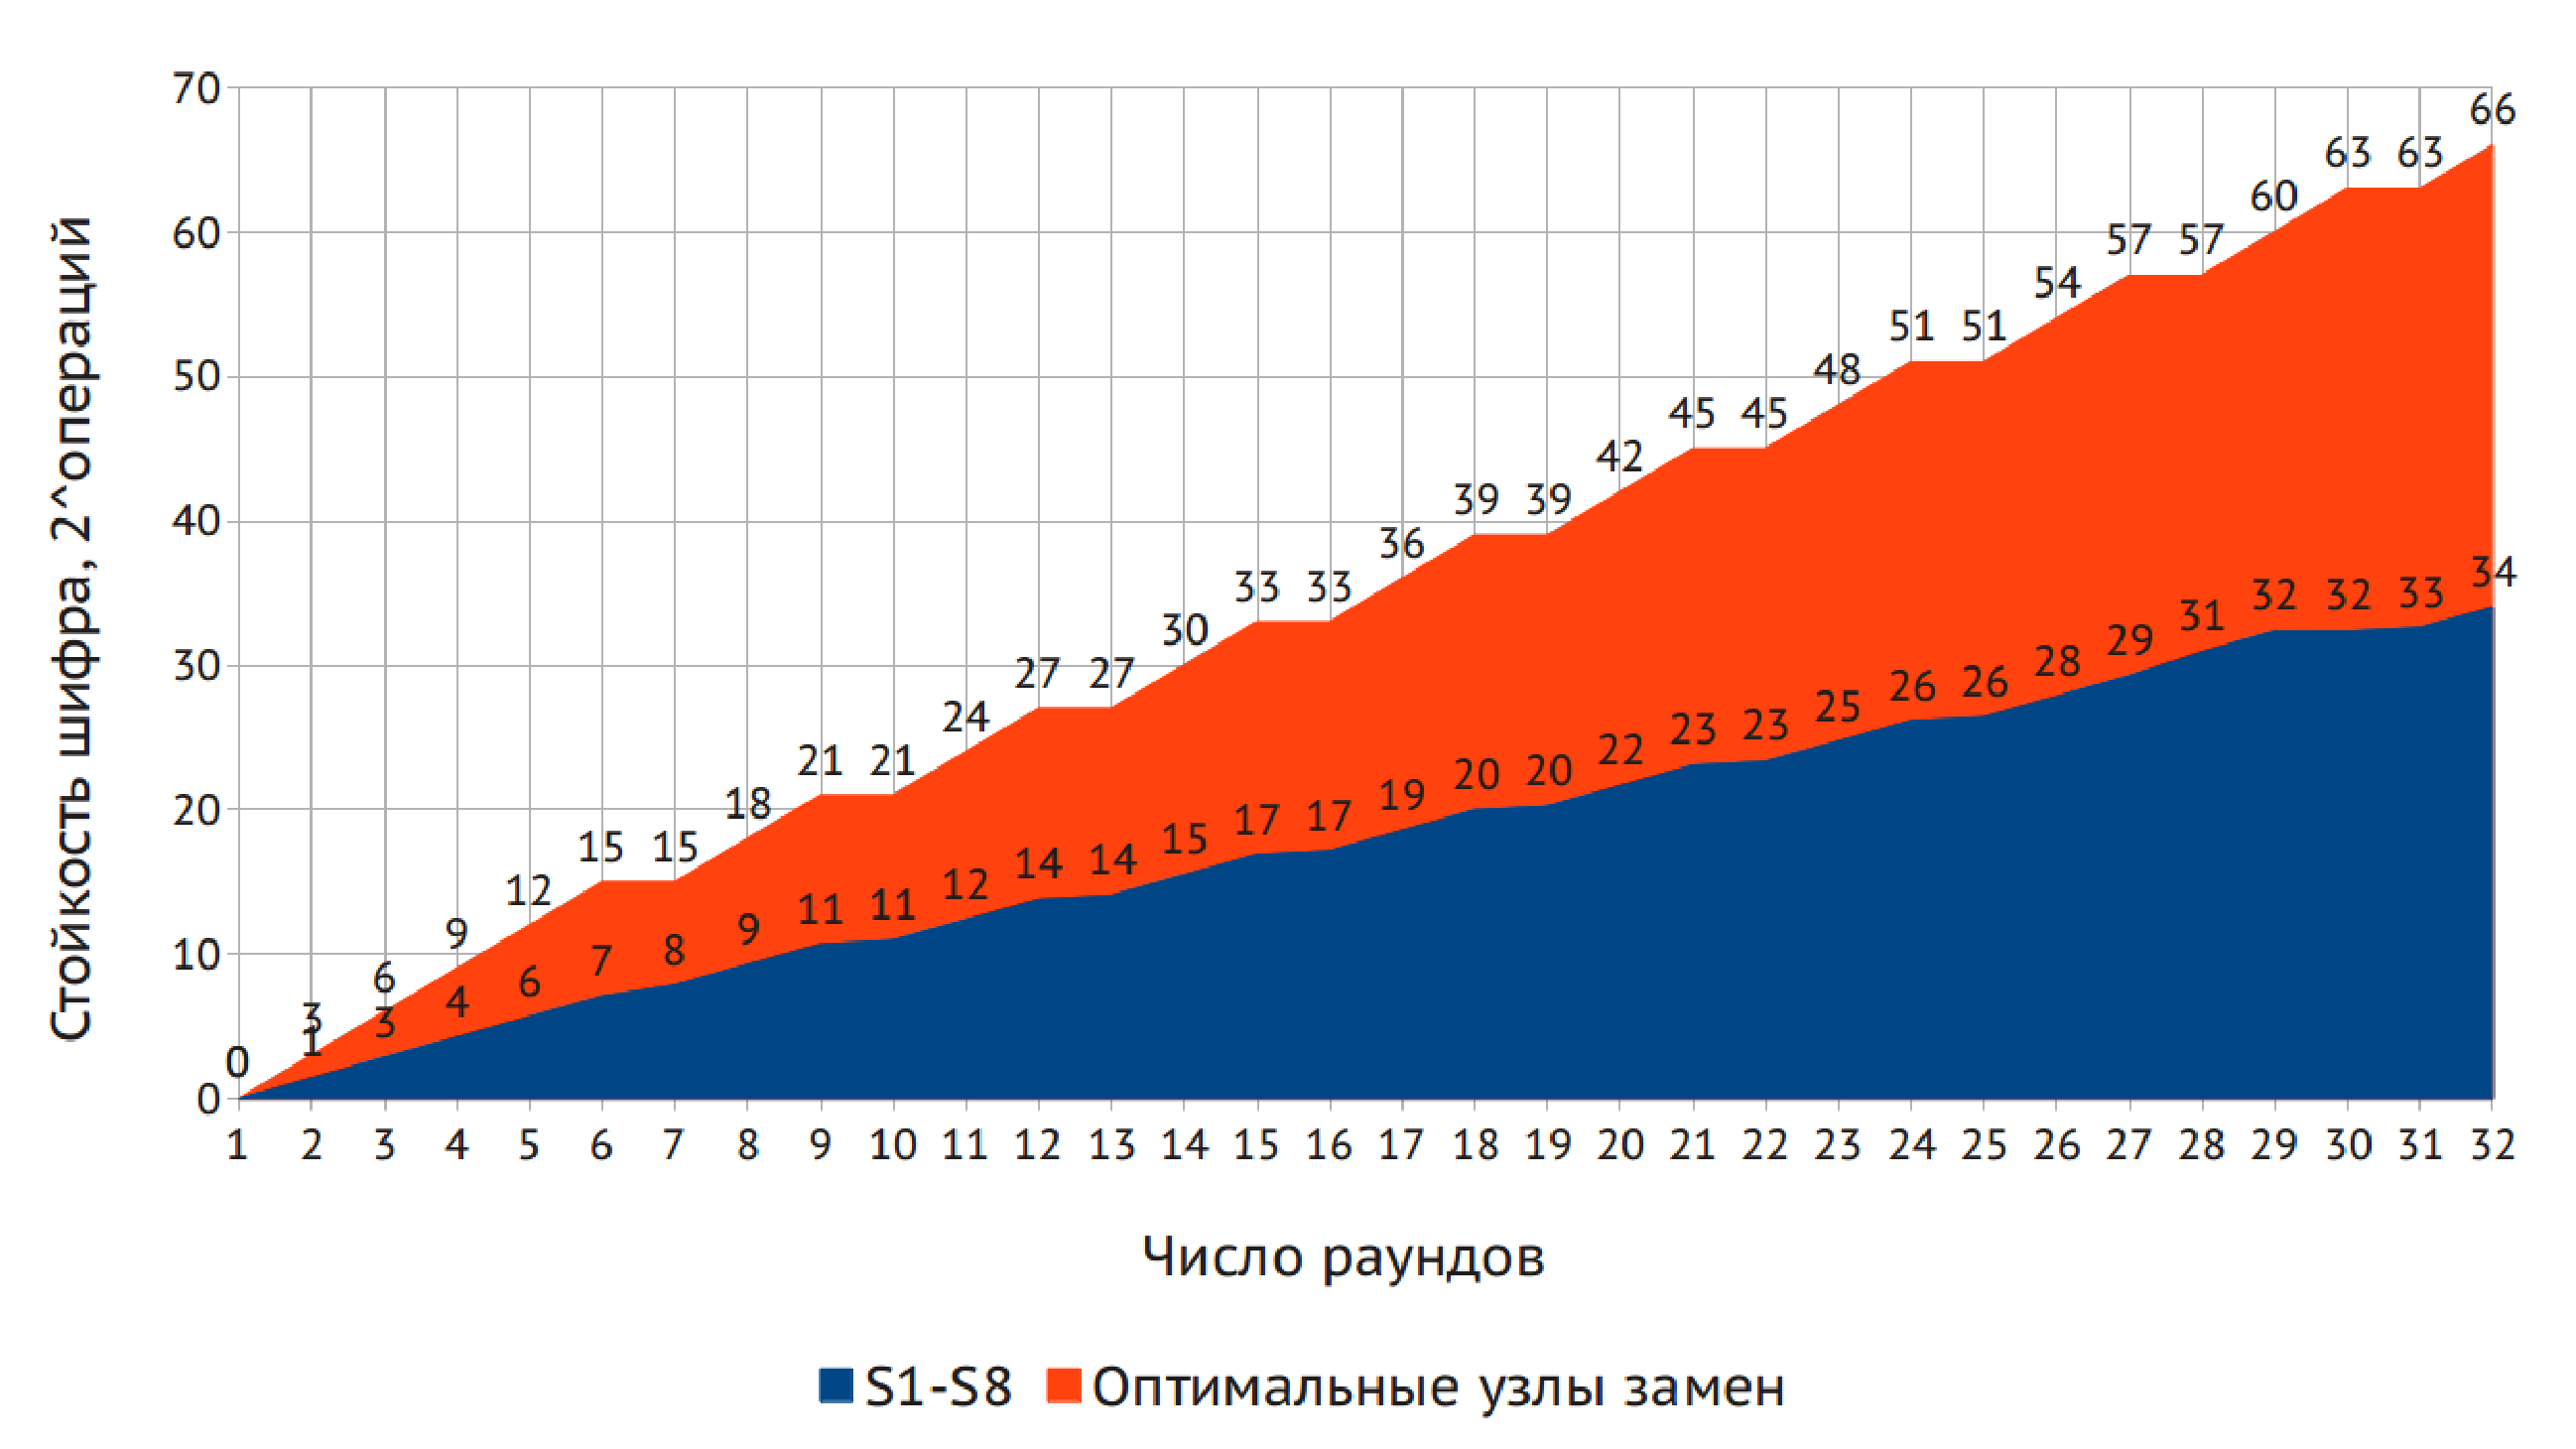
\includegraphics[width=10cm]{GOST_diff_efficiency.eps}
    \end{figure}

\end{frame}


\begin{frame}{Эффективность ГОСТ~28147-89. \\ Стойкость к линейному криптоанализу}

    \begin{figure}
        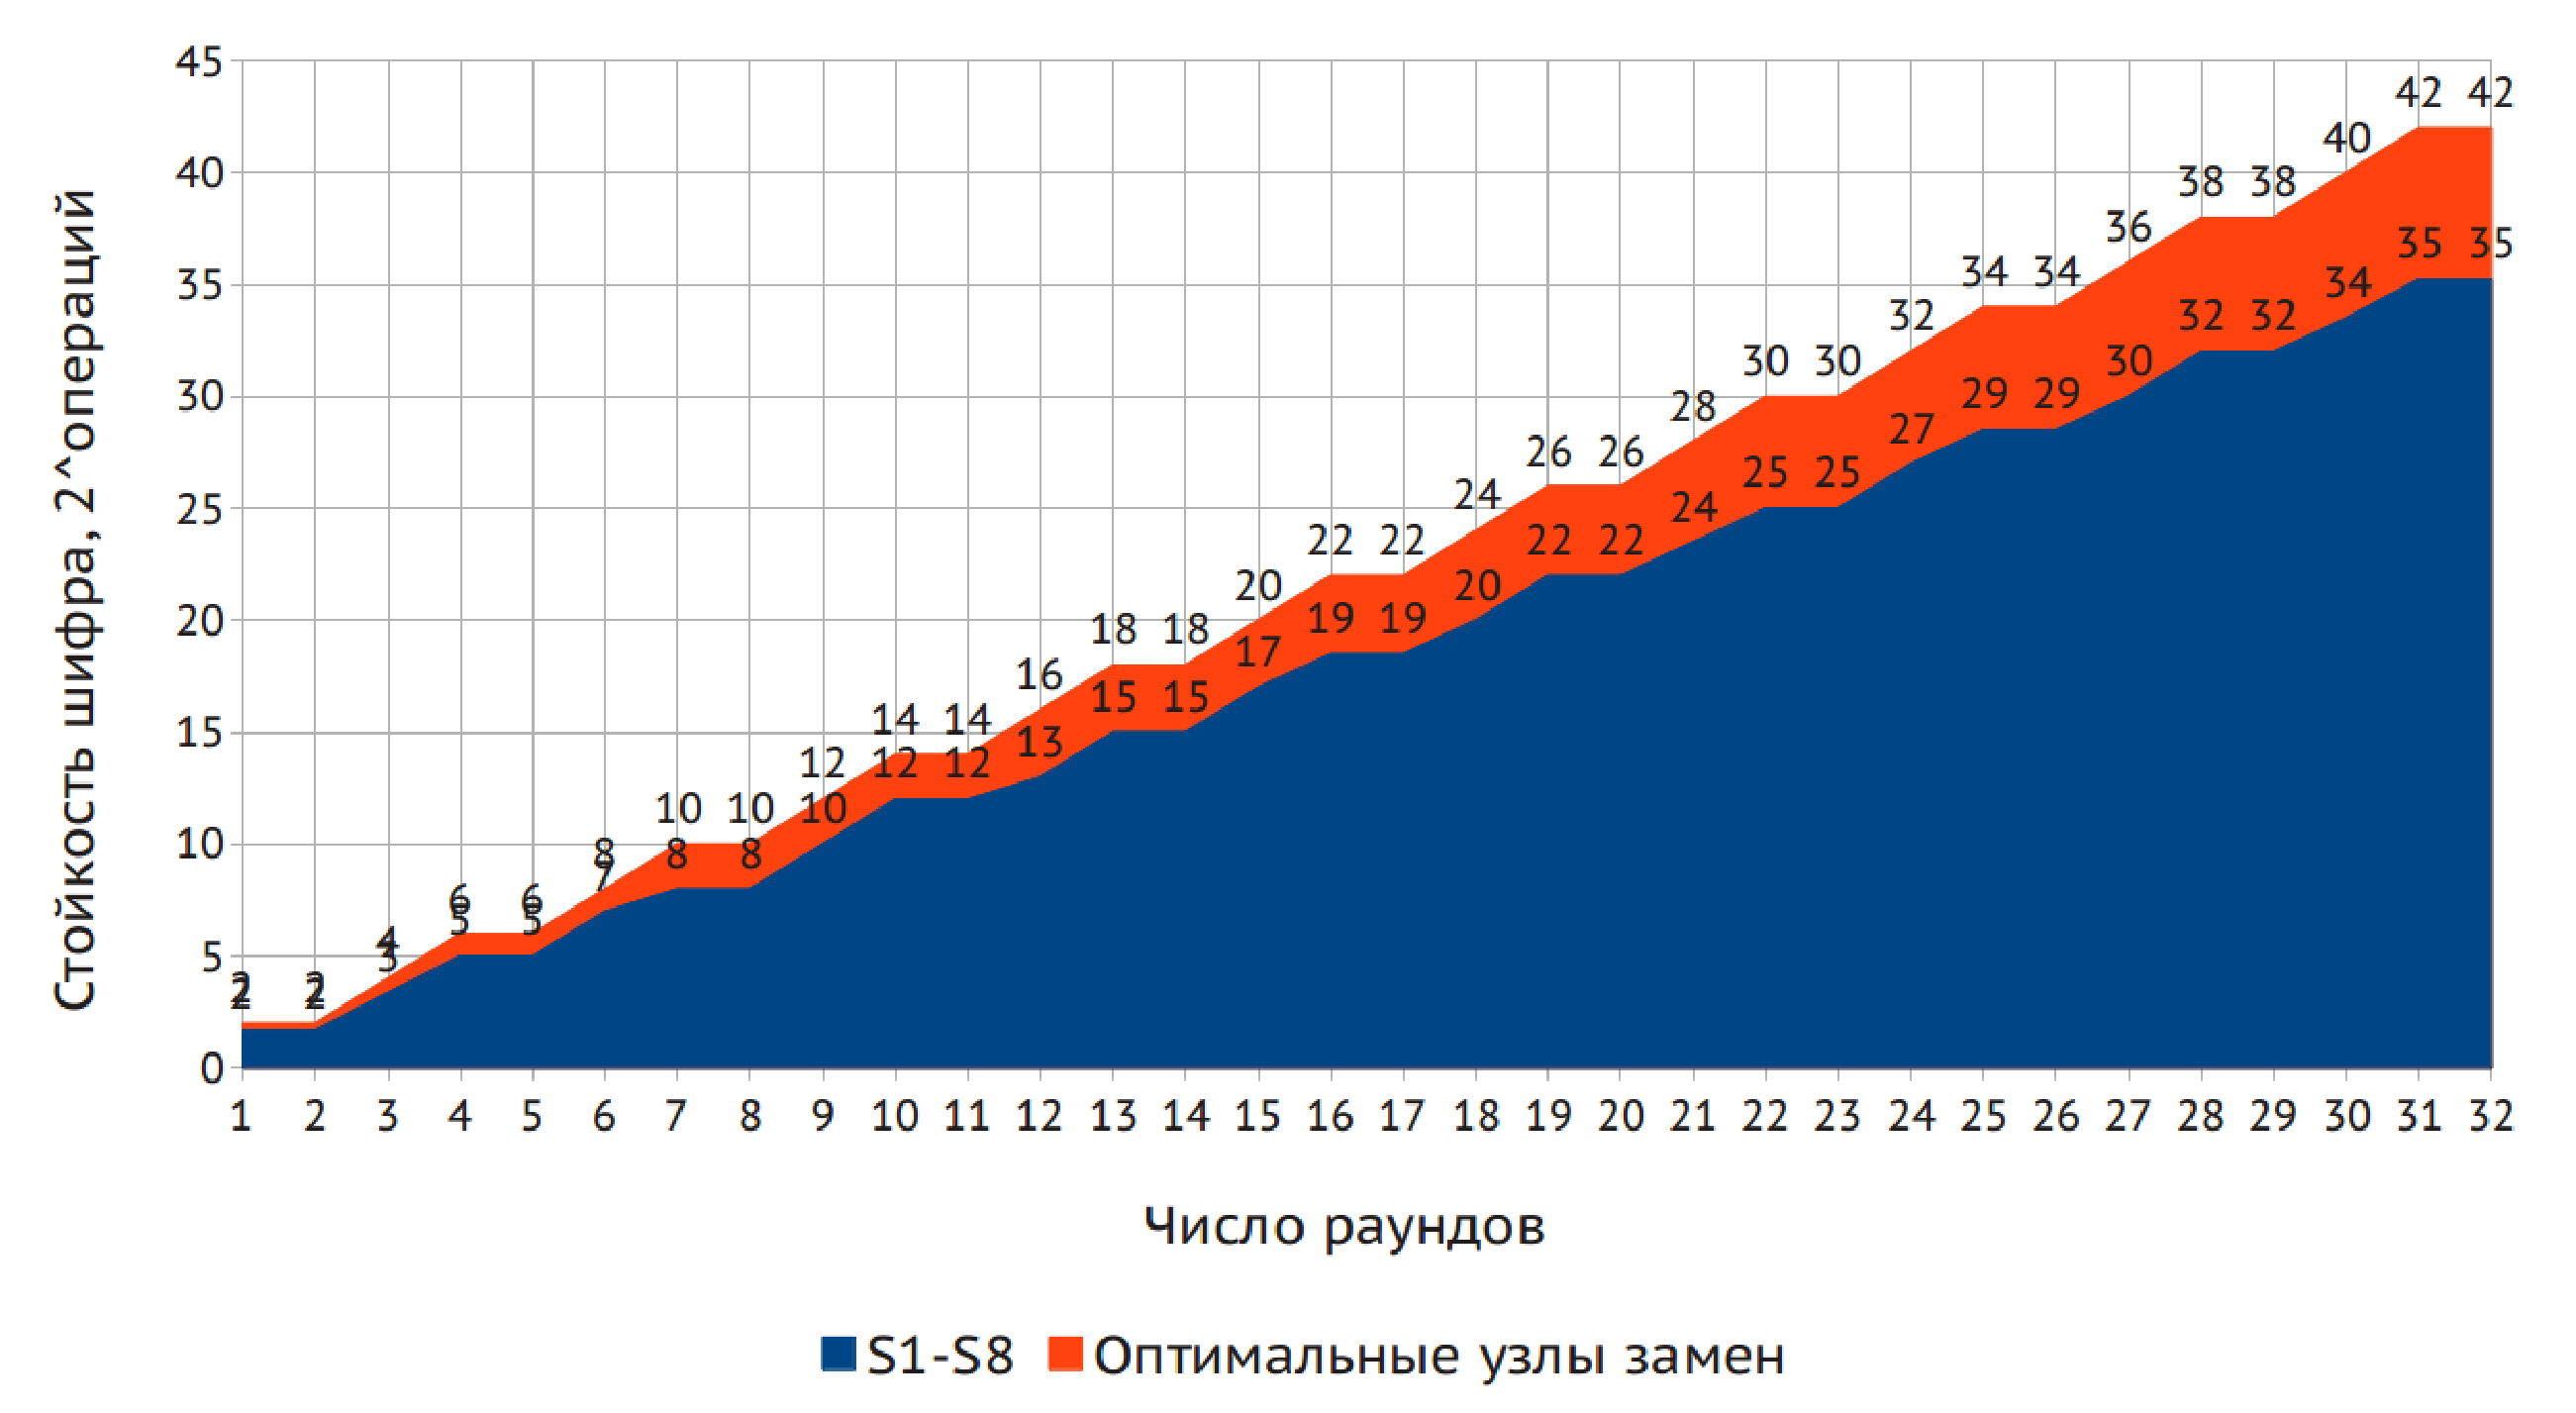
\includegraphics[width=10cm]{GOST_linear_efficiency.eps}
    \end{figure}

\end{frame}


\begin{frame}{Оценка поизводительности формирования S-блоков методом имитации
отжига}

    \begin{figure}
        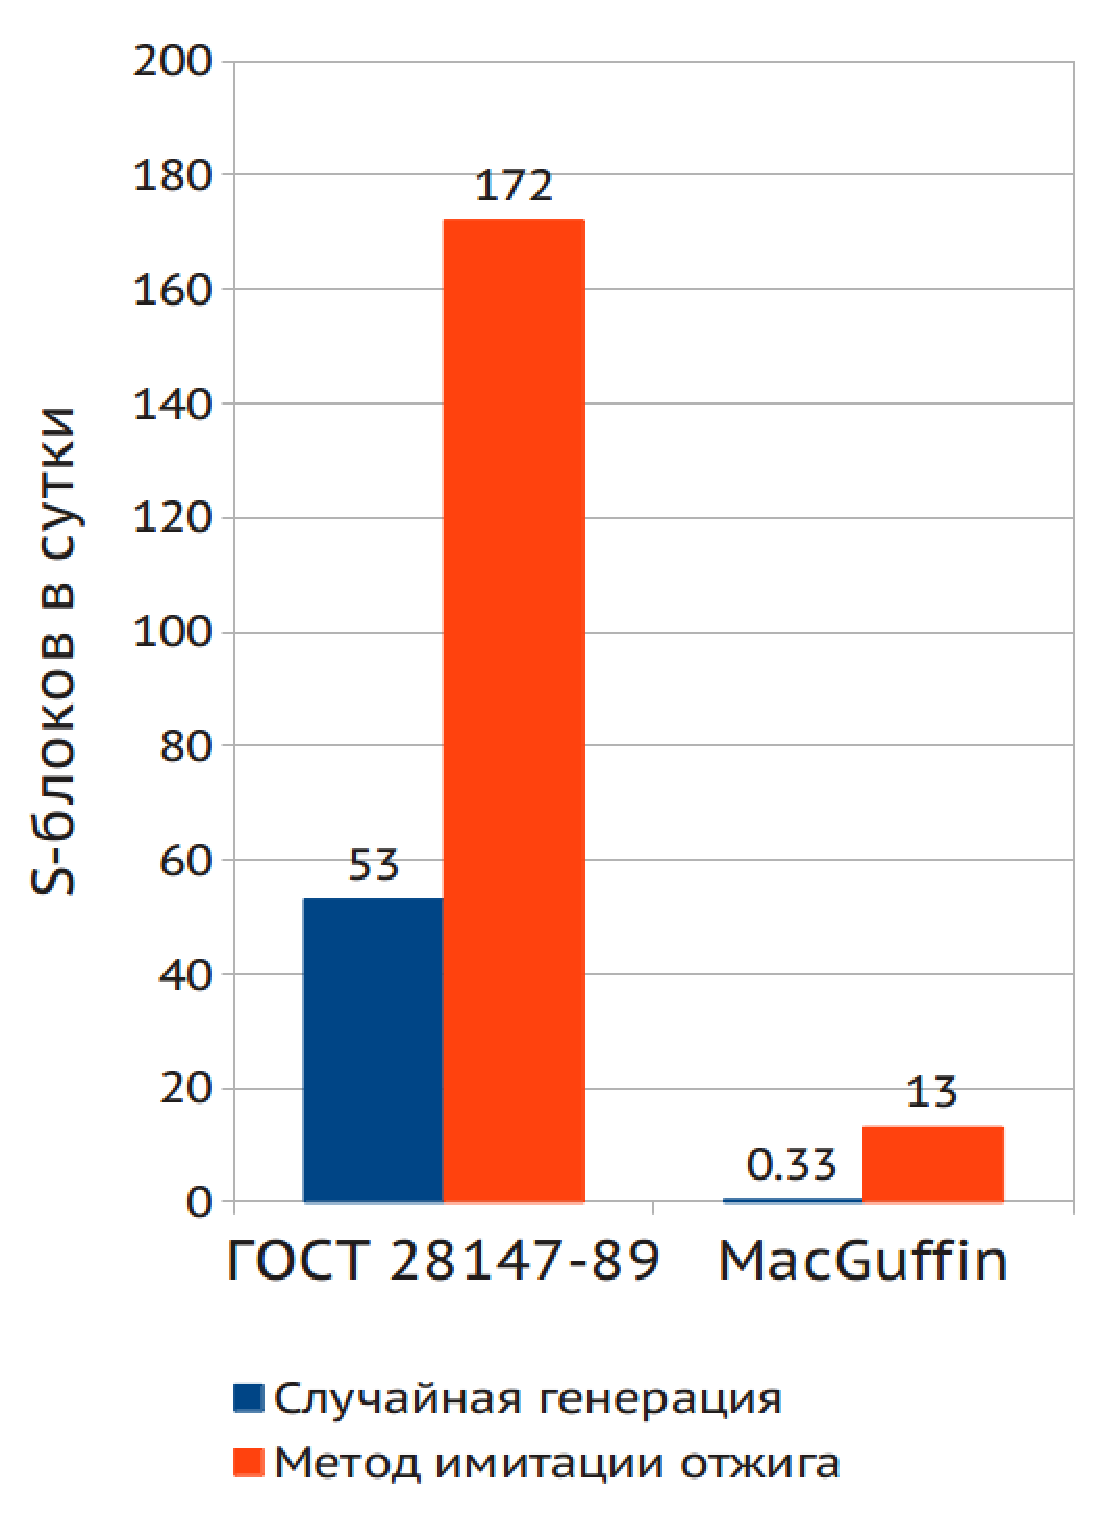
\includegraphics[width=4.2cm]{annealing_performance.eps}
        \hspace{1cm}
        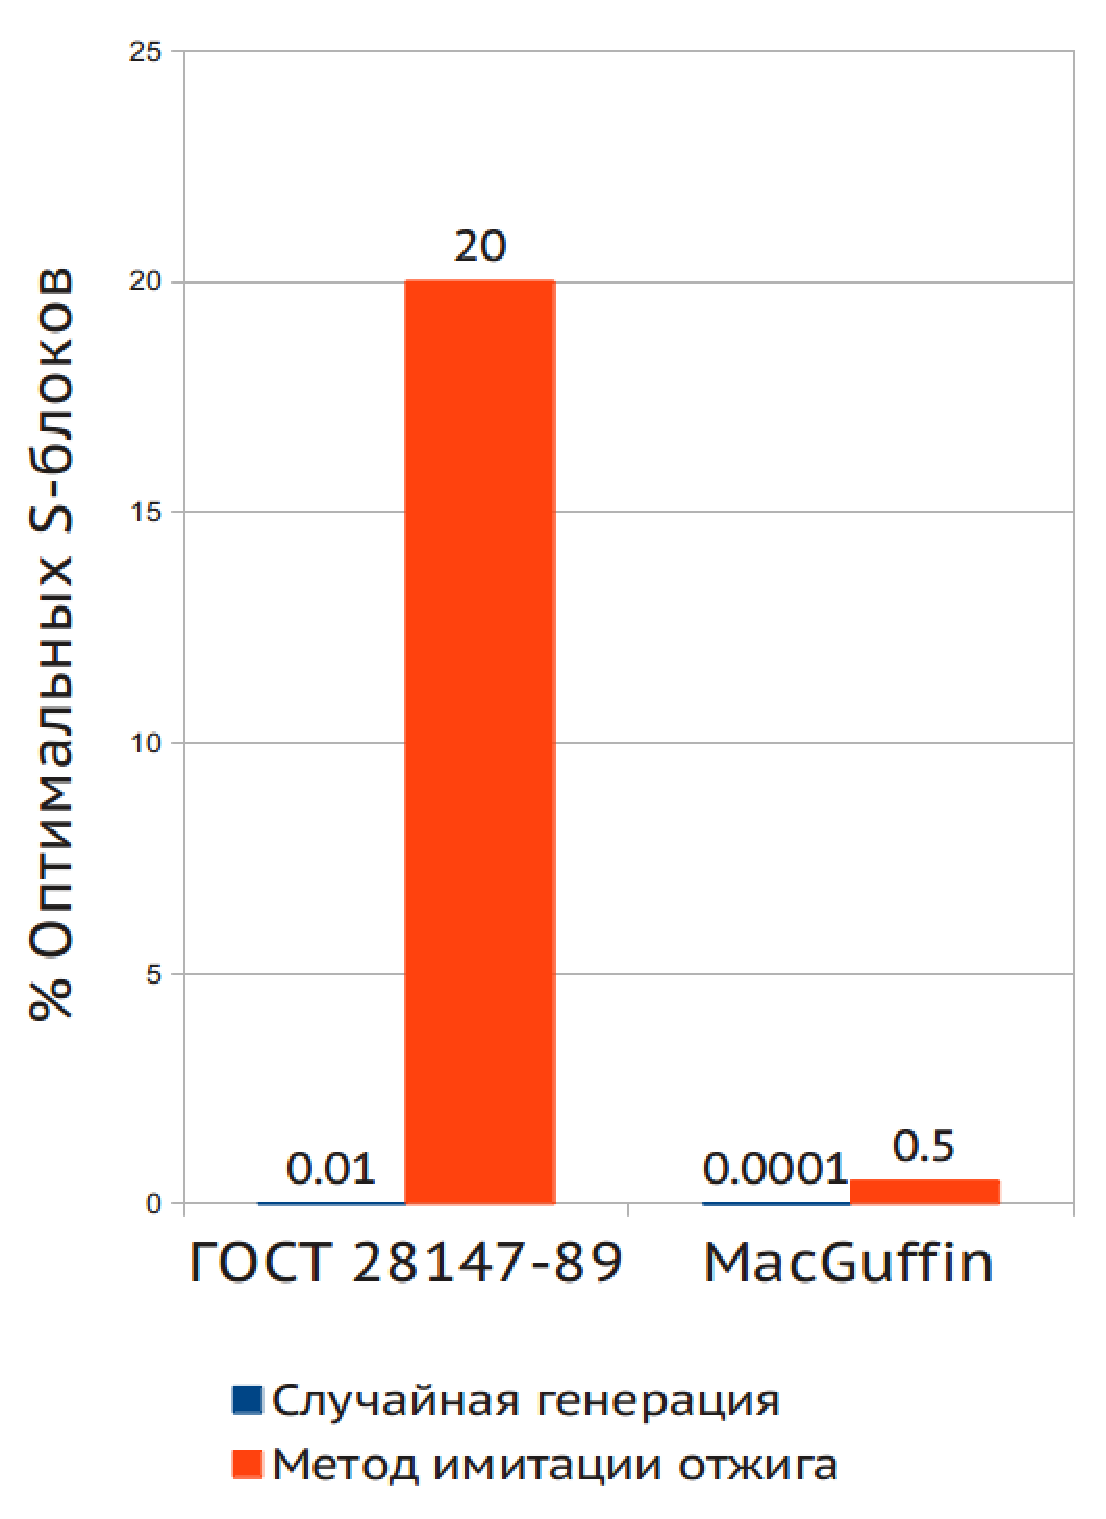
\includegraphics[width=4.2cm]{annealing_performance_percent.eps}
    \end{figure}

\end{frame}


\begin{frame}{Охрана труда и безопасность в чрезвычайных ситуациях}

    \begin{itemize}

        \item Разработаны меры по охране труда в НИЛ с углублённой обработкой вопроса расчёта необходимой площади световых проёмов в помещении НИЛ.
        
        \item Суммарная расчётная площадь световых проёмов составляет 4,3 $\text{м}^2$, в то время как практическая площадь составляет 8 $\text{м}^2$.

    \end{itemize}

\end{frame} 


\begin{frame}{Выводы}

    \begin{itemize}

        \item Исследован и улучшен метод имитации отжига.

        \item Получены наглядные экпериментальные результаты повышения эффективности шифрования при использовании оптимальных S-блоков, сформированных методом имитации отжига.

        \item Оценена производительность метода имитации отжига относительно метода случайной генерации.

    \end{itemize}

\end{frame} 


\begin{frame}{}

    \begin{center}
        \LARGE{Спасибо за внимание.}
    \end{center}

\end{frame}

\end{document}
